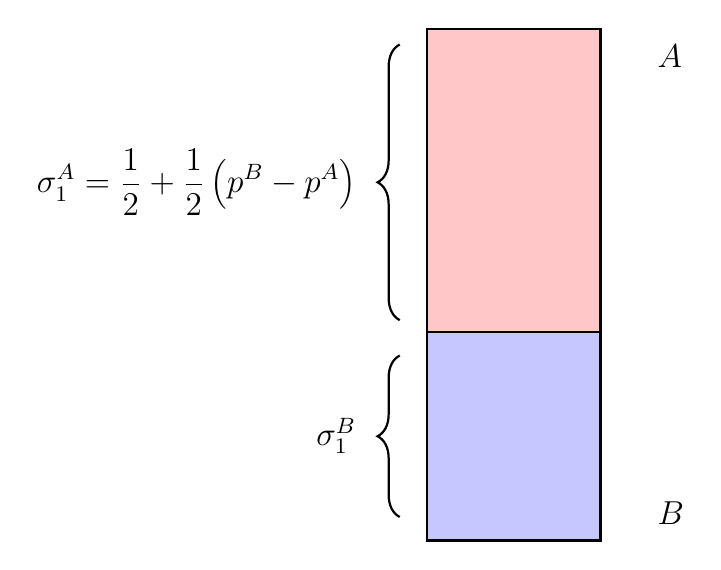
\begin{tikzpicture}[
    every node/.style={font=\large}
]

% Main rectangle
\fill[red!22] (0,2.65) rectangle (2.2,6.5);
\fill[blue!22] (0,0) rectangle (2.2,2.65);
\draw[thick] (0,0) rectangle (2.2,6.5);

% Divider between A and B
\draw[thick] (0,2.65) -- (2.2,2.65);

% Labels A and B
\node[right] at (2.8,6.15) {$A$};
\node[right] at (2.8,0.35) {$B$};

% Braces on left
\draw[
    decorate,
    decoration={brace, amplitude=8pt},
    thick
]
(-0.35,2.8) -- (-0.35,6.3)
node[midway,left=12pt]
{$\displaystyle \sigma_1^A=\frac{1}{2}
  +\frac{1}{2}\left(p^B-p^A\right)$};

\draw[
    decorate,
    decoration={brace, amplitude=8pt},
    thick
]
(-0.35,0.3) -- (-0.35,2.35)
node[midway,left=12pt] {$\sigma_1^B$};

\end{tikzpicture}
